\section{Results}
\label{sec:results}

All tables and figures in this section are generated by \texttt{analysis/figures.py} from the files in \texttt{results/}.
At the time of writing they show the \ResultsSource{}; captions name the source of each item.
The Gemma pilot stopped at 1{,}536 questions in the original order only, so Gemma appears in Figure~\ref{fig:curves} but not yet in the depth tables.

\begin{table}[t]
\centering\small\setlength{\tabcolsep}{4pt}
\begin{tabular}{lrrrrr}
\toprule
Model & $L$ & $n$ & Acc. & $d_{\mathrm{soft}}$ & $\ell^*_{\mathrm{cyc}}/L$ \\
\midrule
Llama-3.1-8B & 32 & 2{,}000 & 0.831 & 0.49 & 0.56 \\
Qwen2.5-7B & 28 & 2{,}000 & 0.810 & 0.62 & 0.79 \\
Gemma-2-9B & -- & -- & -- & -- & -- \\
\bottomrule
\end{tabular}

\caption{Accuracy (gold content top-1 at layer $L$) and median relative depth of correctly answered questions. Source: \SrcModels{}.}
\label{tab:models}
\end{table}

\begin{figure*}[t]
\centering
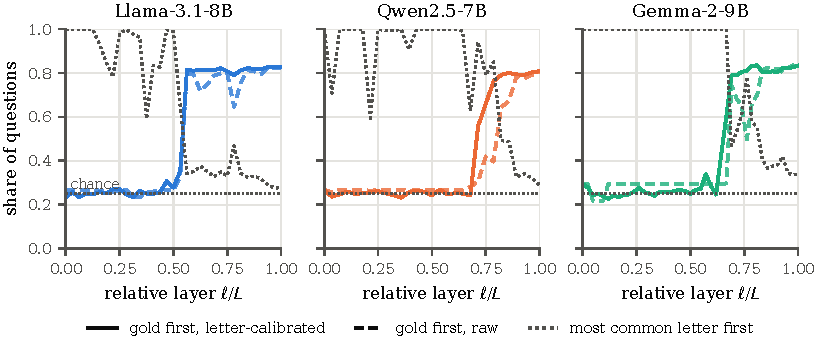
\includegraphics[width=\textwidth]{figures/layer_curves.pdf}
\caption{Logit lens, by relative layer. Coloured lines: share of questions whose gold answer is ranked first, from the raw restricted softmax (dashed) and after subtracting each letter's mean log-probability at that layer (solid). Grey dotted: share of questions on which the single most common letter is ranked first. The black dotted line is chance. Source: \SrcCurves{}.}
\label{fig:curves}
\end{figure*}

\subsection{Where answers crystallize}

Figure~\ref{fig:curves} shows the letter bias and the transition.
Until about half of the depth in Llama and about two thirds in Qwen and Gemma, one letter is ranked first on most questions and the gold answer is ranked first at chance rate.
The share of correct rankings then rises within a few layers to near its final value.
Removing the letter prior makes little difference before this transition and moves the rise slightly earlier, mainly in Qwen; it matters most for per-question depths, where a question whose gold sits at the favoured letter would otherwise be counted as correct from the first layer.
Table~\ref{tab:models} and Figure~\ref{fig:depth} give the depth of correct answers.
\todoresult{Describe the depth distributions per model from the full run: medians of $d_{\mathrm{soft}}$, whether the three models differ in relative depth, and how tuned-lens depths compare to logit-lens depths (tuned lens expected earlier).}

\begin{figure}[t]
\centering
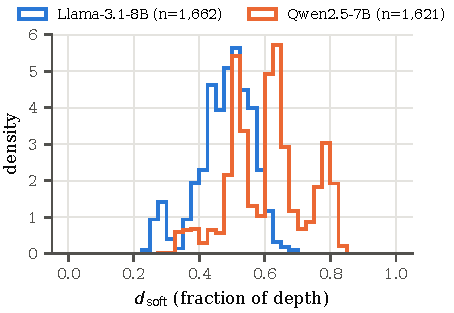
\includegraphics[width=\columnwidth]{figures/depth_distribution.pdf}
\caption{Distribution of $d_{\mathrm{soft}}$ over correctly answered questions. Source: \SrcDist{}.}
\label{fig:depth}
\end{figure}

\subsection{Reliability and choice of metric}

\begin{figure}[t]
\centering
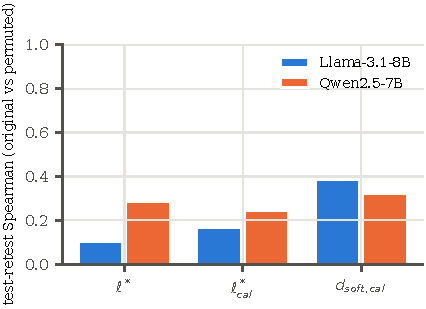
\includegraphics[width=\columnwidth]{figures/reliability.pdf}
\caption{Reliability of the depth metrics on questions correct in both halves or orders. Source: \SrcRel{}.}
\label{fig:reliability}
\end{figure}

Figure~\ref{fig:reliability} reports reliability per metric.
In the pilot, single-order first-correct-layer metrics had test-retest Spearman correlations between 0.10 and 0.28 across the two option orders, and the continuous calibrated depth between 0.32 and 0.39.
\todoresult{split-half reliabilities from the full run for all five metrics and three models, and the outcome of the preregistered rule.}

\subsection{Depth and entity documentation}

\begin{table*}[t]
\centering\small
\begin{tabular}{lccccr}
\toprule
Model & Entity freq. & Holm $p$ & State freq. & Perm.\ $p$ & $n$ \\
\midrule
Llama-3.1-8B & -0.24 [-0.42{,} -0.06] & 0.028 & -0.05 [-0.21{,} +0.11] & 0.58 & 1{,}401 \\
Qwen2.5-7B & +0.18 [-0.07{,} +0.44] & 0.816 & -0.03 [-0.17{,} +0.11] & 0.71 & 1{,}342 \\
Gemma-2-9B & \multicolumn{5}{c}{--} \\
\bottomrule
\end{tabular}

\caption{Effect of one standard deviation of entity frequency (raw log count) and of state frequency on the primary depth metric, in layers, with 95\% confidence intervals (OLS, standard errors clustered by state, all controls). Holm $p$ is adjusted across the five depth metrics. Perm.\ $p$ is the state-label permutation test for state frequency. Source: \SrcEffects{}.}
\label{tab:effects}
\end{table*}

\begin{figure}[t]
\centering
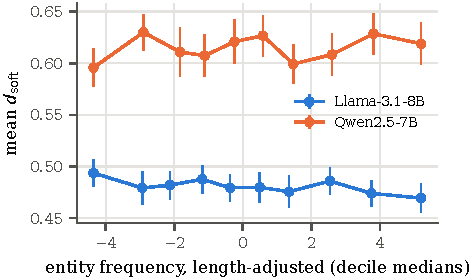
\includegraphics[width=\columnwidth]{figures/frequency.pdf}
\caption{Mean $d_{\mathrm{soft}}$ by decile of length-adjusted entity frequency, with 95\% intervals. Uncontrolled; the tests in Table~\ref{tab:effects} include all controls. Source: \SrcFreq{}.}
\label{fig:freq}
\end{figure}

Table~\ref{tab:effects} and Figure~\ref{fig:freq} report H1 and H2.
In the pilot, which is exploratory and not part of the preregistered test, the entity effect had opposite signs in the two models it covered, and state frequency had no detectable effect.
\todoresult{H1 outcome per the preregistered criteria (positive, null with the equivalence bound, opposite, or inconclusive), with the effect per model in layers per SD; the length-adjusted and pageviews robustness checks; the tuned-lens readout.}
\todoresult{H2 outcome from the permutation test; per-state medians for Maharashtra and Bihar and the extremes.}

\subsection{Activation patching}

\begin{figure}[t]
\centering
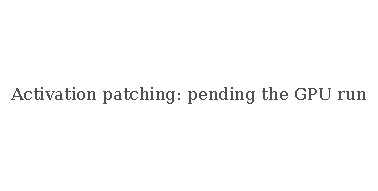
\includegraphics[width=\columnwidth]{figures/patching.pdf}
\caption{Median recovery of the clean logit difference when the clean final-token residual is patched in at each relative layer. Source: \SrcPatch{}.}
\label{fig:patch}
\end{figure}

\todoresult{Number of valid patched questions per model; the layer at which median recovery crosses 0.5; H3 Spearman correlation between patching depth and $d_{\mathrm{soft}}$ with its interval; sensitivity at thresholds 0.3 and 0.7.}
